% --- TurboQuant ---
\begin{frame}[plain]
  \centering
  \vfill
  {\LARGE\bfseries TurboQuant}
  \vfill
\end{frame}

\begin{frame}{TurboQuant: Problem and Motivation}
    \begin{itemize}\itemsep0.28em
      \item[\textcolor{red}{$\blacktriangleright$}] \textbf{Vector quantization (VQ):} compress high-dimensional vectors while controlling \textbf{distortion} of their geometry.
      \begin{itemize}
      \item[\textcolor{red}{$\blacktriangleright$}] Enhances vector search and KV cache compression.
      \end{itemize}
      \item[\textcolor{red}{$\blacktriangleright$}] Prior practical schemes often fall \textbf{short of optimal} distortion--rate scaling.
      \item[\textcolor{red}{$\blacktriangleright$}] TurboQuant shrinks what inference \emph{stores} rather than the model itself: the \textbf{KV cache} during decoding, and the \textbf{embedding vectors} of a search index. Model weights are not its target.
      \item[\textcolor{red}{$\blacktriangleright$}] Reported quality: neutral at \textbf{3.5 bits} per channel for the KV cache, with marginal degradation at 2.5 bits.
      \item[\textcolor{red}{$\blacktriangleright$}] Applies to any model at inference time with no offline preparation or calibration data.
    \end{itemize}
\end{frame}

\begin{frame}{TurboQuant: What ``Near-Optimal Distortion Rate'' Means}
  \begin{itemize}\itemsep0.4em
    \item[\textcolor{red}{$\blacktriangleright$}] For a budget of $b$ bits per coordinate, no quantizer whatsoever can push the mean squared error below a fixed floor; the paper proves that floor is of order $1/4^{b}$.
    \item[\textcolor{red}{$\blacktriangleright$}] TurboQuant's own distortion is shown to sit within a constant factor of at most $\sqrt{3}\pi/2 \approx 2.7$ of that floor, simultaneously for every bit-width and every dimension.
    \item[\textcolor{red}{$\blacktriangleright$}] The guarantee is worst-case and \textbf{data-oblivious}: it holds without a calibration set and without a codebook fitted to the data, which is what allows the quantizer to run online.
    \item[\textcolor{red}{$\blacktriangleright$}] So ``near-optimal'' is a proved bound on MSE distortion, not a benchmark score.
  \end{itemize}
  \vspace{0.3em}
  {\scriptsize Zandieh, Daliri, Hadian \& Mirrokni, ``TurboQuant: Online Vector Quantization with Near-optimal Distortion Rate,'' \href{https://arxiv.org/abs/2504.19874}{arXiv:2504.19874}.}
\end{frame}

\begin{frame}{TurboQuant: How It Works}
  \begin{itemize}\itemsep0.28em
    \item[\textcolor{red}{$\blacktriangleright$}] TurboQuant works in \textbf{two stages:}
      \begin{itemize}
        \item \textbf{Stage 1: random rotation, then scalar quantization.} Randomly rotating a vector spreads its mass evenly, so its coordinates become nearly independent and each follows the same known distribution. That lets a single \textbf{MSE-optimal scalar quantizer} be applied coordinate by coordinate, spending most of the bit budget well without any codebook fitted to the data.
        \item \textbf{Stage 2: removing the inner-product bias with QJL.} An MSE-optimal quantizer is biased when its output is used inside a \emph{dot product}, which is exactly what attention computes. TurboQuant spends one remaining bit on a \textbf{QJL (Quantized Johnson--Lindenstrauss)} transform of the residual, which cancels that bias and makes the estimated attention scores unbiased.
      \end{itemize}
    \item[\textcolor{red}{$\blacktriangleright$}] \textbf{PolarQuant} is a companion method from the same group, not a stage of TurboQuant: it quantizes vectors through a polar transformation and serves here as one of the baselines TurboQuant is measured against.
  \end{itemize}
  \vspace{0.2em}
  {\scriptsize Zandieh \& Mirrokni, ``TurboQuant: Redefining AI efficiency with extreme compression,'' Google Research Blog (2026). \href{https://research.google/blog/turboquant-redefining-ai-efficiency-with-extreme-compression/}{Article}.}
\end{frame}

\begin{frame}{TurboQuant: Experiments and Results}
  \centering
  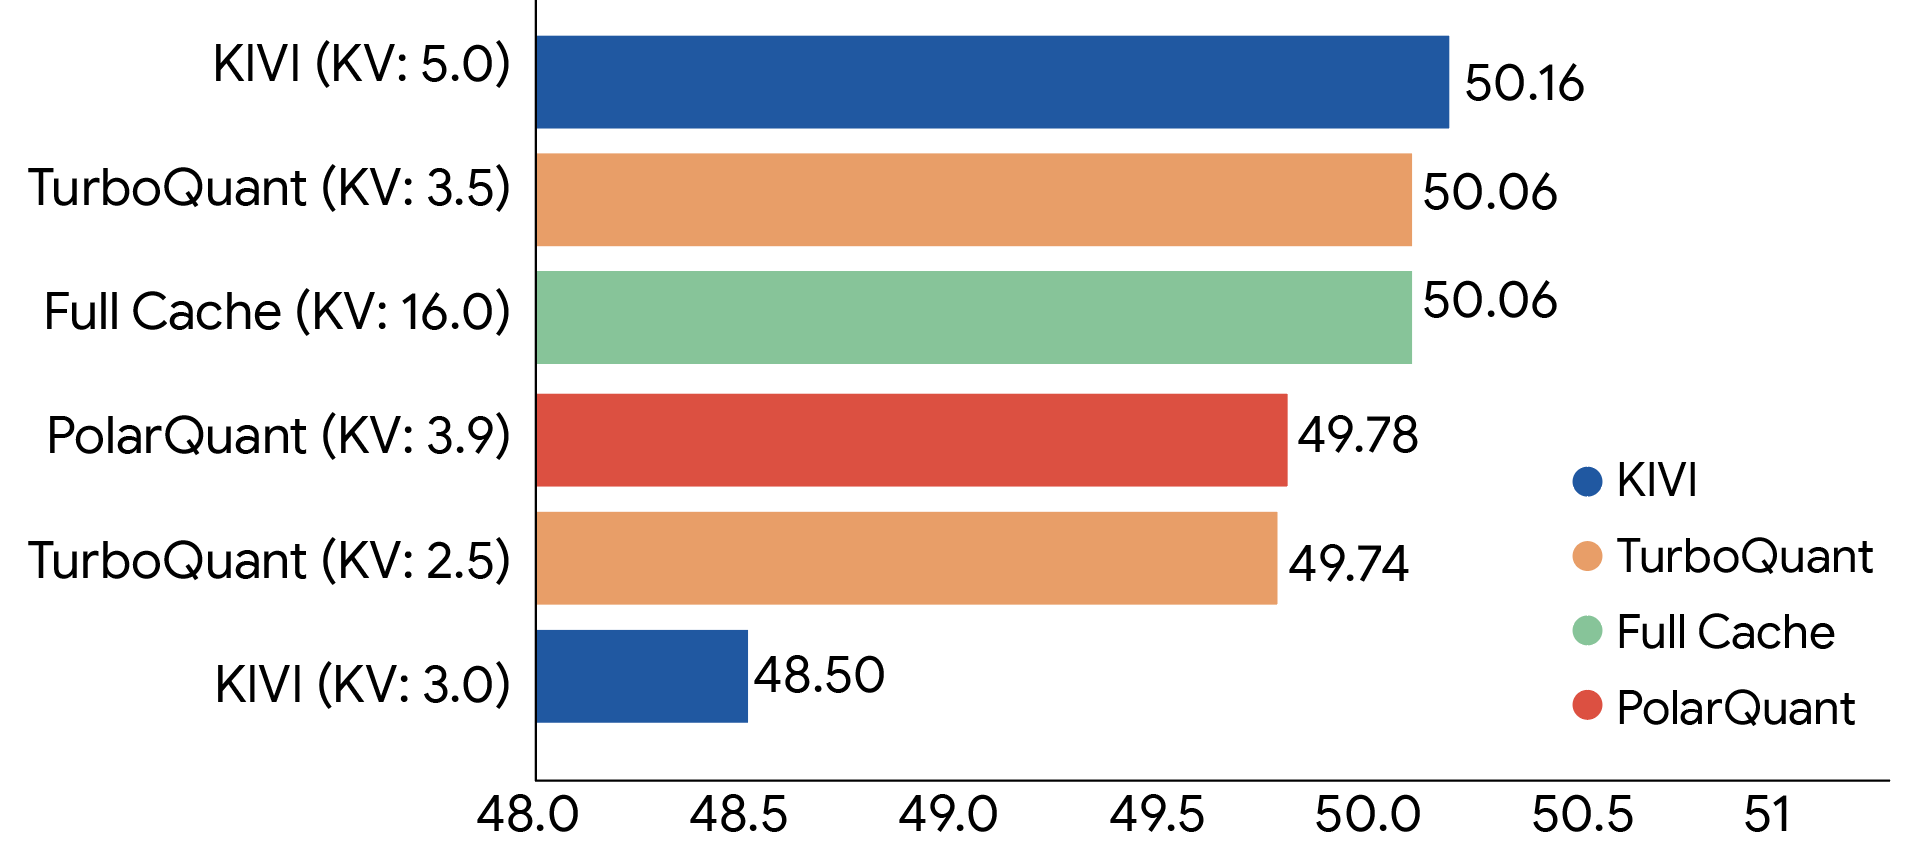
\includegraphics[width=\linewidth,height=0.82\textheight,keepaspectratio]{images/inference-optimisation/google_research_turboquant_longbench_llama.png}\\[0.35em]
  {\scriptsize KV cache compression on the LongBench benchmark (QA, code generation, summarization) with Llama-3.1-8B-Instruct: TurboQuant vs.\ PolarQuant and KIVI; bit-widths in brackets. Reference: Google Research Blog.}
\end{frame}

\begin{frame}{TurboQuant: Experiments and Results}
  \centering
  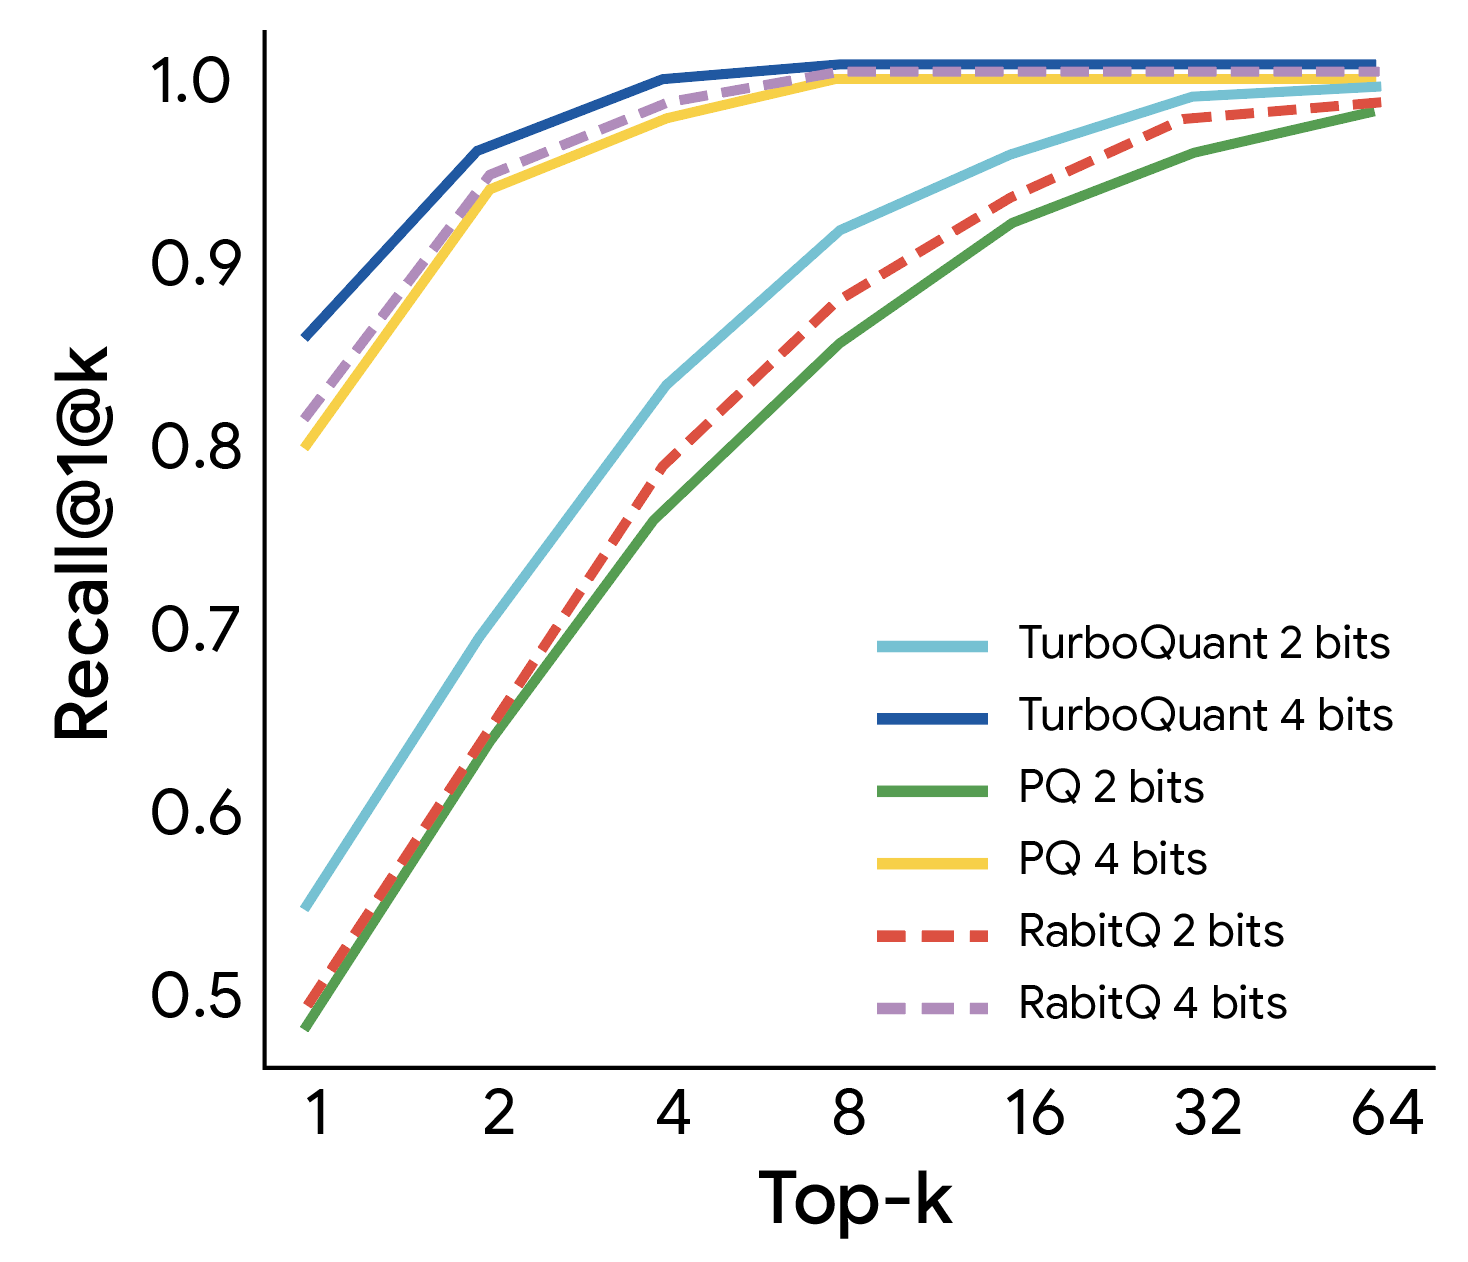
\includegraphics[width=\linewidth,height=0.82\textheight,keepaspectratio]{images/inference-optimisation/google_research_turboquant_glove_recall.png}\\[0.35em]
  {\scriptsize \textbf{1@$k$ recall} on GloVe ($d{=}200$): TurboQuant vs.\ Product Quantization (PQ) and RaBitQ. Reference: Google Research Blog.}
\end{frame}
